\section{Spark::Sp\-Reference$<$ Class\-Type $>$ Class Template Reference}
\label{classSpark_1_1SpReference}\index{Spark::SpReference@{Spark::SpReference}}
{\tt \#include $<$Sp\-Reference.h$>$}

Collaboration diagram for Spark::Sp\-Reference$<$ Class\-Type $>$:\begin{figure}[H]
\begin{center}
\leavevmode
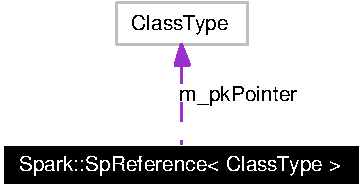
\includegraphics[width=104pt]{classSpark_1_1SpReference__coll__graph}
\end{center}
\end{figure}


\subsection{Detailed Description}
\subsubsection*{template$<$class Class\-Type$>$ class Spark::Sp\-Reference$<$ Class\-Type $>$}

Reference class with garbage collection for supporting shared objects. 

Definition at line 31 of file Sp\-Reference.h.\subsection*{Public Member Functions}
\begin{CompactItemize}
\item 
{\bf Sp\-Reference} (Class\-Type $\ast$pk\-Object=0)
\begin{CompactList}\small\item\em Construction:. \item\end{CompactList}\item 
{\bf Sp\-Reference} (const {\bf Sp\-Reference} \&rk\-Sp\-Reference)
\item 
{\bf $\sim$Sp\-Reference} ()
\item 
{\bf operator Class\-Type $\ast$} () const
\begin{CompactList}\small\item\em Conversions:. \item\end{CompactList}\item 
Class\-Type \& {\bf operator $\ast$} () const
\item 
Class\-Type $\ast$ {\bf operator $\rightarrow$ } () const
\item 
{\bf Sp\-Reference} \& {\bf operator=} (const {\bf Sp\-Reference} \&rk\-Sp\-Reference)
\begin{CompactList}\small\item\em Assignment:. \item\end{CompactList}\item 
{\bf Sp\-Reference} \& {\bf operator=} (Class\-Type $\ast$pk\-Object)
\item 
bool {\bf operator==} (Class\-Type $\ast$pk\-Object) const
\begin{CompactList}\small\item\em Comparison:. \item\end{CompactList}\item 
bool {\bf operator!=} (Class\-Type $\ast$pk\-Object) const
\item 
bool {\bf operator==} (const {\bf Sp\-Reference} \&rk\-Sp\-Reference) const
\item 
bool {\bf operator!=} (const {\bf Sp\-Reference} \&rk\-Sp\-Reference) const
\end{CompactItemize}
\subsection*{Protected Attributes}
\begin{CompactItemize}
\item 
Class\-Type $\ast$ {\bf m\_\-pk\-Pointer}
\begin{CompactList}\small\item\em Internal Data:. \item\end{CompactList}\end{CompactItemize}


\subsection{Constructor \& Destructor Documentation}
\index{Spark::SpReference@{Spark::Sp\-Reference}!SpReference@{SpReference}}
\index{SpReference@{SpReference}!Spark::SpReference@{Spark::Sp\-Reference}}
\subsubsection{\setlength{\rightskip}{0pt plus 5cm}template$<$class Class\-Type$>$ {\bf Spark::Sp\-Reference}$<$ Class\-Type $>$::{\bf Sp\-Reference} (Class\-Type $\ast$ {\em pk\-Object} = {\tt 0})}\label{classSpark_1_1SpReference_a0}


Construction:. 

Definition at line 74 of file Sp\-Reference.h.\index{Spark::SpReference@{Spark::Sp\-Reference}!SpReference@{SpReference}}
\index{SpReference@{SpReference}!Spark::SpReference@{Spark::Sp\-Reference}}
\subsubsection{\setlength{\rightskip}{0pt plus 5cm}template$<$class Class\-Type$>$ {\bf Spark::Sp\-Reference}$<$ Class\-Type $>$::{\bf Sp\-Reference} (const {\bf Sp\-Reference}$<$ Class\-Type $>$ \& {\em rk\-Sp\-Reference})}\label{classSpark_1_1SpReference_a1}


Definition at line 82 of file Sp\-Reference.h.\index{Spark::SpReference@{Spark::Sp\-Reference}!~SpReference@{$\sim$SpReference}}
\index{~SpReference@{$\sim$SpReference}!Spark::SpReference@{Spark::Sp\-Reference}}
\subsubsection{\setlength{\rightskip}{0pt plus 5cm}template$<$class Class\-Type$>$ {\bf Spark::Sp\-Reference}$<$ Class\-Type $>$::$\sim${\bf Sp\-Reference} ()}\label{classSpark_1_1SpReference_a2}


Definition at line 90 of file Sp\-Reference.h.

\subsection{Member Function Documentation}
\index{Spark::SpReference@{Spark::Sp\-Reference}!operator *@{operator $\ast$}}
\index{operator *@{operator $\ast$}!Spark::SpReference@{Spark::Sp\-Reference}}
\subsubsection{\setlength{\rightskip}{0pt plus 5cm}template$<$class Class\-Type$>$ Class\-Type \& {\bf Spark::Sp\-Reference}$<$ Class\-Type $>$::operator $\ast$ () const}\label{classSpark_1_1SpReference_a4}


Definition at line 103 of file Sp\-Reference.h.\index{Spark::SpReference@{Spark::Sp\-Reference}!operator ClassType *@{operator ClassType $\ast$}}
\index{operator ClassType *@{operator ClassType $\ast$}!Spark::SpReference@{Spark::Sp\-Reference}}
\subsubsection{\setlength{\rightskip}{0pt plus 5cm}template$<$class Class\-Type$>$ {\bf Spark::Sp\-Reference}$<$ Class\-Type $>$::operator Class\-Type $\ast$ () const}\label{classSpark_1_1SpReference_a3}


Conversions:. 

Definition at line 97 of file Sp\-Reference.h.\index{Spark::SpReference@{Spark::Sp\-Reference}!operator"!=@{operator"!=}}
\index{operator"!=@{operator"!=}!Spark::SpReference@{Spark::Sp\-Reference}}
\subsubsection{\setlength{\rightskip}{0pt plus 5cm}template$<$class Class\-Type$>$ bool {\bf Spark::Sp\-Reference}$<$ Class\-Type $>$::operator!= (const {\bf Sp\-Reference}$<$ Class\-Type $>$ \& {\em rk\-Sp\-Reference}) const}\label{classSpark_1_1SpReference_a11}


Definition at line 165 of file Sp\-Reference.h.\index{Spark::SpReference@{Spark::Sp\-Reference}!operator"!=@{operator"!=}}
\index{operator"!=@{operator"!=}!Spark::SpReference@{Spark::Sp\-Reference}}
\subsubsection{\setlength{\rightskip}{0pt plus 5cm}template$<$class Class\-Type$>$ bool {\bf Spark::Sp\-Reference}$<$ Class\-Type $>$::operator!= (Class\-Type $\ast$ {\em pk\-Object}) const}\label{classSpark_1_1SpReference_a9}


Definition at line 153 of file Sp\-Reference.h.\index{Spark::SpReference@{Spark::Sp\-Reference}!operator->@{operator-$>$}}
\index{operator->@{operator-$>$}!Spark::SpReference@{Spark::Sp\-Reference}}
\subsubsection{\setlength{\rightskip}{0pt plus 5cm}template$<$class Class\-Type$>$ Class\-Type $\ast$ {\bf Spark::Sp\-Reference}$<$ Class\-Type $>$::operator $\rightarrow$  () const}\label{classSpark_1_1SpReference_a5}


Definition at line 109 of file Sp\-Reference.h.\index{Spark::SpReference@{Spark::Sp\-Reference}!operator=@{operator=}}
\index{operator=@{operator=}!Spark::SpReference@{Spark::Sp\-Reference}}
\subsubsection{\setlength{\rightskip}{0pt plus 5cm}template$<$class Class\-Type$>$ {\bf Sp\-Reference}$<$ Class\-Type $>$ \& {\bf Spark::Sp\-Reference}$<$ Class\-Type $>$::operator= (Class\-Type $\ast$ {\em pk\-Object})}\label{classSpark_1_1SpReference_a7}


Definition at line 131 of file Sp\-Reference.h.\index{Spark::SpReference@{Spark::Sp\-Reference}!operator=@{operator=}}
\index{operator=@{operator=}!Spark::SpReference@{Spark::Sp\-Reference}}
\subsubsection{\setlength{\rightskip}{0pt plus 5cm}template$<$class Class\-Type$>$ {\bf Sp\-Reference}$<$ Class\-Type $>$ \& {\bf Spark::Sp\-Reference}$<$ Class\-Type $>$::operator= (const {\bf Sp\-Reference}$<$ Class\-Type $>$ \& {\em rk\-Sp\-Reference})}\label{classSpark_1_1SpReference_a6}


Assignment:. 

Definition at line 115 of file Sp\-Reference.h.\index{Spark::SpReference@{Spark::Sp\-Reference}!operator==@{operator==}}
\index{operator==@{operator==}!Spark::SpReference@{Spark::Sp\-Reference}}
\subsubsection{\setlength{\rightskip}{0pt plus 5cm}template$<$class Class\-Type$>$ bool {\bf Spark::Sp\-Reference}$<$ Class\-Type $>$::operator== (const {\bf Sp\-Reference}$<$ Class\-Type $>$ \& {\em rk\-Sp\-Reference}) const}\label{classSpark_1_1SpReference_a10}


Definition at line 159 of file Sp\-Reference.h.\index{Spark::SpReference@{Spark::Sp\-Reference}!operator==@{operator==}}
\index{operator==@{operator==}!Spark::SpReference@{Spark::Sp\-Reference}}
\subsubsection{\setlength{\rightskip}{0pt plus 5cm}template$<$class Class\-Type$>$ bool {\bf Spark::Sp\-Reference}$<$ Class\-Type $>$::operator== (Class\-Type $\ast$ {\em pk\-Object}) const}\label{classSpark_1_1SpReference_a8}


Comparison:. 

Definition at line 147 of file Sp\-Reference.h.

\subsection{Member Data Documentation}
\index{Spark::SpReference@{Spark::Sp\-Reference}!m_pkPointer@{m\_\-pkPointer}}
\index{m_pkPointer@{m\_\-pkPointer}!Spark::SpReference@{Spark::Sp\-Reference}}
\subsubsection{\setlength{\rightskip}{0pt plus 5cm}template$<$class Class\-Type$>$ Class\-Type$\ast$ {\bf Spark::Sp\-Reference}$<$ Class\-Type $>$::{\bf m\_\-pk\-Pointer}\hspace{0.3cm}{\tt  [protected]}}\label{classSpark_1_1SpReference_p0}


Internal Data:. 

Definition at line 66 of file Sp\-Reference.h.

The documentation for this class was generated from the following file:\begin{CompactItemize}
\item 
{\bf Sp\-Reference.h}\end{CompactItemize}
